% This is LLNCS.DEM the demonstration file of
% the LaTeX macro package from Springer-Verlag
% for Lecture Notes in Computer Science,
% version 2.4 for LaTeX2e as of 16. April 2010
%
\documentclass{llncs}
%
\usepackage{graphicx}
\usepackage{makeidx}  % allows for indexgeneration
%
\begin{document}
%
\frontmatter          % for the preliminaries
%
%\pagestyle{headings}  % switches on printing of running heads
%
%
\title{The Micromapping Model of Computation; the Foundation for Optimized Execution of Eclipse QVTc/QVTr/UMLX.}
%
\titlerunning{Micromapping Model of Computation}  % abbreviated title (for running head)
%                                     also used for the TOC unless
%                                     \toctitle is used
%
\author{Edward D. Willink}
%
\authorrunning{Edward D. Willink} % abbreviated author list (for running head)
%
%%%% list of authors for the TOC (use if author list has to be modified)
\tocauthor{Edward Willink}
%
\institute{Willink Transformations Ltd., Reading, UK,\\
\email{ed \_at\_ willink.me.uk}
}

\maketitle              % typeset the title of the contribution

\begin{abstract}
It is 14 years since the first UMLX paper and 10 years since the QVT 1.0 specification was published. No useable UMLX implementation has appeared. QVTr implementations have been disappointing. The Eclipse QVTd project can now offer editing, optimization, execution and Java code generation for QVTc, QVTr and UMLX. This paper outlines the Micromapping Model of Computation used by the optimizations.
\keywords{declarative model transformation, QVTc, QVTr, UMLX, optimization}
\end{abstract}
%

\section{Introduction}

The QVT specification introduced one imperative language, QVTo, and two declarative languages, QVTc and QVTr, as the solution to the early enthusiasm for model to model transformation. Only QVTo has a flourishing implementation. QVTc was never implemented despite the `c' suggesting it is a core that `o' and `r' extend. The two QVTr implementations have not prospered.

The Eclipse QVTd project \cite{Eclipse-QVTd} has provided QVTc and QVTr editors for many years, but it is only recently\footnote{As part of the Eclipse Neon release in June 2016.} that any execution functionality has been available.

UMLX \cite{UMLX} was proposed a little before QVT \cite{QVT-1.0}. UMLX extends UML-like object diagrams to specify the object patterns to be transformed. However three successive implementation attempts for UMLX foundered on the lack of an execution capability. UMLX and QVTr have now evolved to share some fairly obvious declarative principles enabling the Eclipse QVTd project to offer graphical UMLX as an interchangeable syntax for textual QVTr.

This paper describes the analyses and transformations that solve the problem; convert UMLX, QVTr and QVTc declarative forms to an optimized imperative representation suitable for interpreted or code generated execution. In Section~\ref{Background}, we contrast an imperative Procedure with a declarative Mapping\footnote{A Mapping is also known as a Relation or a Rule} before introducing a Micromapping and its inter-Connection as the basis for the compile-time analysis described in Section~\ref{Analysis}. Section~\ref{Results} presents some results, Section~\ref{Related Work} related work and Section~\ref{Status} the current status. Section~\ref{Conclusion} concludes.

\section{Background}\label{Background}

The familiar way in which a procedure interacts with its caller and objects is shown at the left of Fig~\ref{fig:FunctionContext}. The example procedure receives a $param1$ parameter value from its caller, and executes, using the parameter to identify $object1$, whose $slot1$ references an $object2$ whose $slot3$ contributes to some computation of a value to be assigned to $slot4$ of $object3$. This is identified by $slot2$ of $object1$. On completion, the procedure returns the $result1$ value. The life cycle of the procedure is shown at the right of Fig~\ref{fig:FunctionContext}; the procedure is called, it executes and returns. If something goes wrong an exception may be thrown.

\begin{figure}
  \begin{center}
    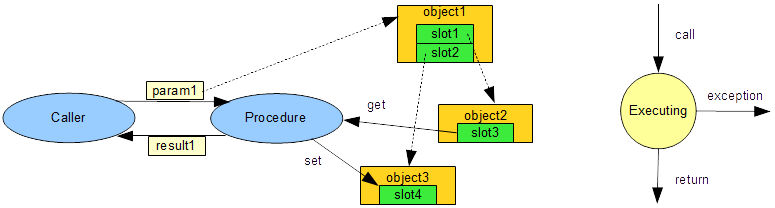
\includegraphics[width=4.5in]{FunctionContext.png}
  \end{center}
  \caption{Example Procedure Interactions and Life Cycle}
  \label{fig:FunctionContext}
\end{figure}

In contrast, the invocation of a declarative transformation mapping need not be explicit. Rather, when objects are available, the mapping is invoked exactly once for each distinct permutation of suitable input objects. The interaction with objects shown at the right of Fig~\ref{fig:MappingContext} is similar to those of a procedure, however the life cycle is more complex. The $invoke$, $exception$ and $success$ transitions correspond to the $call$, $exception$ and $return$ transitions of a procedure. The $failure$ transition occurs when the mapping's predicates or guards are not satisfied; no execution is required. The $not$-$ready$ transition occurs for a premature access to an object or slot; the execution cannot proceed. A $re$-$invoke$ may be attempted once the accessed object or slot is available.

\begin{figure}
	\begin{center}
		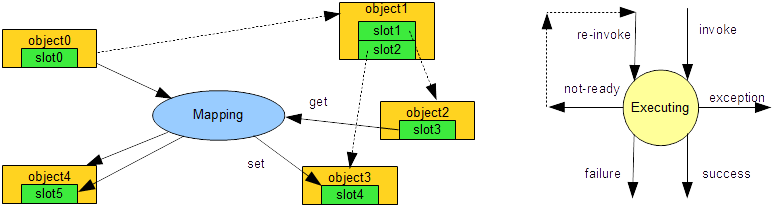
\includegraphics[width=4.5in]{MappingContext.png}
	\end{center}
	\caption{Example Declarative Mapping Interactions and Life Cycle}
	\label{fig:MappingContext}
\end{figure}


%Functions provide many opportunities for careless programmers to have a hard time debugging their failure to ensure that all accessed objects are ready before a function is executed. In contrast declarative mappings impose a heavy responsibility on the run-time to keep track of the transitive readiness of all accessed object slots.

%A further difference between procedures and mappings occurs for repeated execution. A procedure executes each repeat to ensure that side effects are repeated. A mapping invocation must detect the repeat in order to re-use the previous results and avoid any repeated model mutation.

Sequencing explicit procedure calls and slot accesses can be a challenging manual programming responsibility. Mappings are invoked automatically when the appropriate object slots are ready eliminating this opportunity for error.

These differences require the run-time for a declarative transformation to be aware of what has executed and which objects and slots are ready. Naively this could make the declarative transformation slower, however the restricted side effects offer significant opportunities for analysis, optimization and so enhanced performance.

\subsection{Micromappings}

The simplest run-time for declarative mappings may just invoke all possible mappings for all possible object permutations, repeating the invocations for $not$-$ready$ slot accesses. This is hideously inefficient. It may not even work since it assumes that there is at least one sequence of mapping executions that yields the required result. However a mapping may group multiple computations, generally to assist human readability. There is no prohibition on one mapping's slot access depending on another mapping's slot assignment and vice-versa, just the common sense prohibition on a pair of mappings such as $X1$ that computes $a = b + 1$ and $X2$ that performs a contradictory computation $b = a + 1$.
 
A mapping such as $X3$ that computes both $b = c + 1$ and $d = a + 1$ does not contradict $X1$ but it conflicts. $X1$ must wait for $X3$ to provide $b$, and $X3$ must wait for $X1$ to provide $a$. Partitioning $X3$ into $X3a$ and $X3b$, one for each computation, removes the conflict; $X1$ can be computed after $X3a$ and before $X3b$. We call these conflict-free partitioned mappings micromappings.

More formally, a micromapping is a guarded atomic computation. It comprises two active life cycle phases, shown in Fig~\ref{fig:MicromappingContext}, a $fragile\ head$ and a $robust\ tail$. The atomic $robust\ tail$ may create or modify objects. The $fragile\ head$ may bypass execution if a predicate is not satisfied or defer execution if a memory access is premature. The $fragile\ head$ may be executed as many times as necessary to obtain the values needed by the $robust\ tail$. Since the $fragile\ head$ makes no changes, there is never any need to roll-back inadvertent changes. The $Waiting$ pre-state and the $Failure$/$Success$ post-states act as mementoes to ensure that repeated invocation can be detected and results re-used.

\begin{figure}
  \begin{center}
    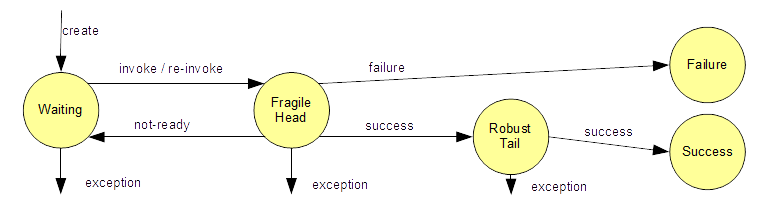
\includegraphics[width=4.75in]{MicromappingContext.png}
  \end{center}
  \caption{Micromapping Execution Life Cycle}
  \label{fig:MicromappingContext}
\end{figure}

A minimal micromapping performs exactly one model mutation to avoid inter-mapping conflict. A more pragmatic and efficient micromapping aggregates multiple non-conflicting changes.

\subsection{Connections}

Each micromapping typically consumes and produces one or more values each with  statically declared type.
%, however a 'kind' may be more elaborate to exploit simple patterns, such as no-children.
Communication between producer and consumer can be managed by a connection so that connections (C*) and micromappings (M*)  form a graph as shown in Fig~\ref{fig:ExecutionContext}. The first layer of connections is primed by a loader, the results are drained by a saver.

\begin{figure}
  \begin{center}
    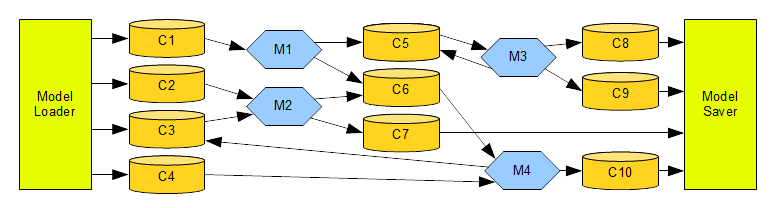
\includegraphics[width=4.75in]{ExecutionContext.png}
  \end{center}
  \caption{Example Micromapping and Connection Data Flow Graph}
  \label{fig:ExecutionContext}
\end{figure}

The graph is directed and mostly acyclic. Acyclic parts are amenable to an efficient overall static schedule such as $for$ $each$ $value$ $in$ $C1$ $do$ $M1$. Cyclic parts require dynamic run-time scheduling that is conveniently orchestrated by ensuring that each connection takes responsibility for creating each distinct invocation of each mapping. Thereafter each micromapping invocation can progress from $Waiting$ to $Success$/$Failure$ under the control of an overall dynamic scheduler.

A procedure just uses its input and returns an output. A micromapping consumes an input value from a connection and may append an output value to another connection. The connection is responsible for invoking all consuming micromappings for each available value, and for accumulating the contributions of all producing micromappings. For micromappings that consume multiple inputs, an invocation occurs for each distinct permutation of the input values.

\subsection{Dependencies}

The example mapping shown in Fig~\ref{fig:MappingContext} has a single input, but as a consequence of object navigation, it also uses three other objects. These are also inputs in so far as they must be available for execution to succeed. We should therefore augment Fig~\ref{fig:ExecutionContext} with additional nodes for each accessed object, and dependency edges for each assignment/access to each of these objects. Fig~\ref{fig:ObjectContext} shows just one such dependency where $M1$ assigns to an $O1.P1$ which is accessed by $M2$. This provides very important information for the static schedule; perform all $M1$ invocations before $M2$ invocations in order to avoid premature $M2$ invocation encountering a $not$-$ready$ for $O1.P1$.

%Further, once $M1$ invocation precedes $M2$, the need for $M2$ to check whether its $O1::P1$ is ready is removed. This saves code, time and memory.

\begin{figure}
  \begin{center}
    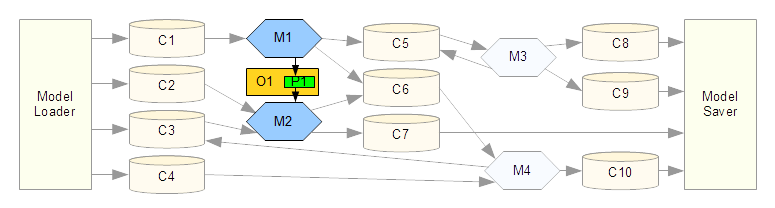
\includegraphics[width=4.75in]{ObjectContext.png}
  \end{center}
  \caption{Example Additional Object Dependency}
  \label{fig:ObjectContext}
\end{figure}

Functions provide no programming assistance to ensure that objects are accessed and updated in a sound order. This provides excellent opportunities for exciting debugging sessions as unintended concurrencies materialize in practice. Declarative mappings eliminate this major practical hazard by requiring slot accesses to wait until the slot is ready. For an OCL-based transformation language, such as QVTc or QVTr, this is possible. For a traditional non-functional programming language such as Java, it is not practical.
%unless some very strong disciplines are informally observed. 

%We will now examine the progressive transformation from source transformations to executable schedules.

\section{Compile-time Analysis and Transformation Chain}\label{Analysis}

The transformation chain of the Eclipse QVTd project is shown in Fig~\ref{fig:architecture}.

\begin{figure}[h]
	\centering
	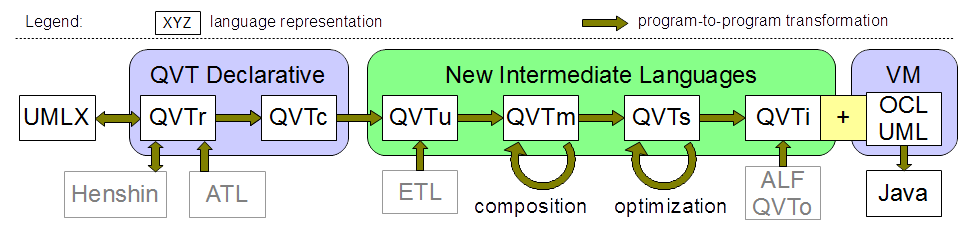
\includegraphics[width=1.0\textwidth]{QVThorizontalAlphabet.png}
	\caption{Progressive transformation architecture for Declarative QVT.}
	\label{fig:architecture}
\end{figure}

\begin{itemize}
	\item UMLX2QVTr graph patterns rewritten as tree patterns
	\item QVTr2QVTc rich concepts rewritten, middle model synthesized
	\item QVTc2QVTu (Unidirectional) irrelevant directions removed
	\item QVTu2QVTm (Minimal) nesting/refinement flattened
	\item QVTm2QVTs (Schedule) micromappings and connections identified
	\item QVTs2QVTi (Imperative) sequential program written
	\item QVTi2Java direct Java code generation
\end{itemize} 

\subsection{Running Example}

In this paper we concentrate on the micromappings, connections and optimizations involving the QVTs representation. We use a very simple example whose metamodel is shown in Fig~\ref{fig:doublylinkedlist}. The example transformation creates a copy of a $DoublyLinkedList$ and its $Element$s reversing the order of the elements in the copy. We will look primarily at the rule that copies one $Element$ and reverses the $source$/$target$ relationship. (The example was presented at EXE 2016 \cite{Willink-EXE2016}.)

\begin{figure}[h]
	\centering
	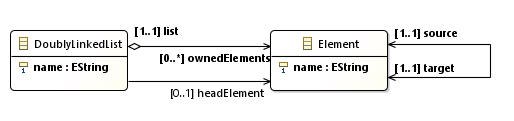
\includegraphics[width=1.0\textwidth]{doublylinkedlist.png}
	\caption{Doubly-Linked List Metamodel.}
	\label{fig:doublylinkedlist}
\end{figure}

The QVTr version shown in Fig~\ref{fig:QVTrelement2element} demonstrates the bidirectional symmetry. Either $forward$ or $reverse$  may be externally  selected as the output domain; the other is the input domain. Each $domain$ clause has a root object and three property values, matched in the input domain, assigned in the output domain. The relationships defined by other mappings are explicit in the $when$ clauses. 
%The QVTr exposition is bidirectional; either $forward$ or $reverse$ domains may be selected as the output, with the other as the input.

\begin{figure}[h]
	\centering
	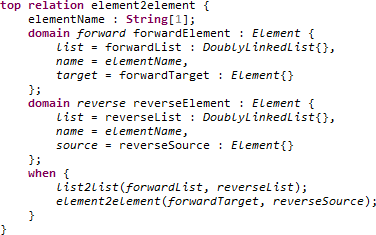
\includegraphics[width=0.6\textwidth]{QVTrelement2element.png}
	\caption{(Manual) QVTr exposition of element2element.}
	\label{fig:QVTrelement2element}
\end{figure}

The corresponding ATL \cite{Eclipse-ATL} exposition of the example shown in Fig~\ref{fig:ATLelement2element} is much more compact but just unidirectional. The relationships established by other mappings occur invisibly as a consequence of two commented implicit invocations of the $resolveTemp$ language facility.

\begin{figure}[h]
	\centering
	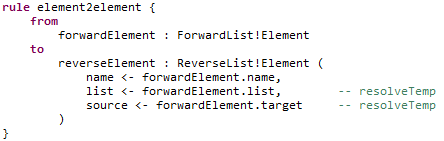
\includegraphics[width=0.7\textwidth]{ATLelement2element.png}
	\caption{(Manual) ATL exposition of element2element.}
	\label{fig:ATLelement2element}
\end{figure}


\subsection{Automated Analysis}

The QVTr2UMLX transformation can be used to autogenerate\footnote{The layout of auto-generated diagrams has been manually improved.} the UMLX exposition of the example shown in Fig~\ref{fig:UMLXelement2element}. This again shows the symmetry of the patterns in the $forward$ and $reverse$ domains, together with explicit invocation of other mappings. The graphics show the patterns more clearly with many graphical decorations automatically derived from the metamodel.

\begin{figure}[h]
	\centering
	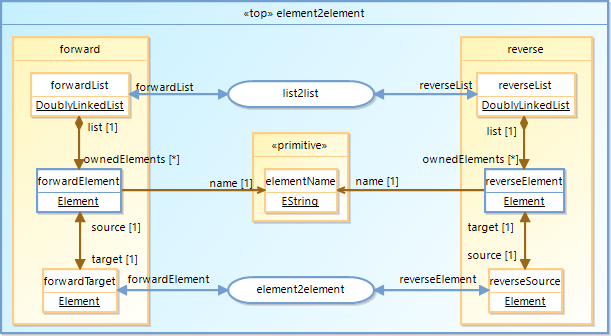
\includegraphics[width=1.0\textwidth]{UMLXelement2element.png}
	\caption{(Automated) UMLX exposition of element2element.}
	\label{fig:UMLXelement2element}
\end{figure}

The brown elements in UMLX are internal to the mapping, whereas blue elements may interact with other mappings. Thus the outer blue box defines the $element2element$ mapping with $forward$, $reverse$ and $primitive$ domains.  The blue $forwardElement$ and $reverseElement$ are the root of each domain whose correspondence may be exploited by another mapping. For this example the $forwardTarget$ and $reverseTarget$ do precisely this through the use of the blue rounded rectangle that is another invocation of $element2element$. Therefore on completion, the $forwardTarget$ (or $reverseSource$) of each invocation of $element2element$ is associated with the $forwardElement$ (or $reverseElement$) of another $element2element$ invocation.

The UMLX exposition demonstrates that declarative model transformations are closely related to graph transformations. It is therefore not surprising that after simplification and conversion to a unidirectional form, the residue of the QVTr AST can be analyzed to identify the object relationships. These are shown in the QVTs representation of Fig~\ref{fig:QVTselement2element}. The QVTs/UMLX similarities are not surprising, so we will concentrate on the differences. 

\begin{figure}[h]
	\centering
	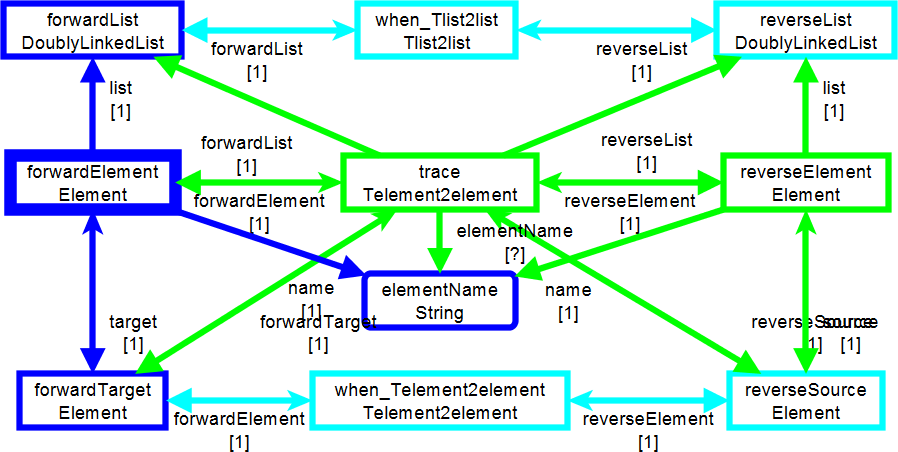
\includegraphics[width=1.0\textwidth]{QVTselement2element.png}
	\caption{(Automated) QVTs exposition of element2element Mapping.}
	\label{fig:QVTselement2element}
\end{figure}

The center traceability column of Fig~\ref{fig:QVTselement2element} has an additional $trace$ node of type $Telement2element$. This is the traceability object that the QVTr2QVTc transformation synthesizes to satisfy the QVTc requirement that all traceability is explicit. Each instance of the trace class corresponds to a distinct invocation of the mapping. Properties of the trace class support the use of OCL navigation expressions to explore the objects matched by a particular mapping invocation. The trace object for one mapping invocation may be referenced by another as occurs for the UMLX invocations of $list2list$ and $element2element$. These are made explicit as further objects of type $Tlist2list$ and $Telement2element$.

The QVTs and UMLX edges correspond to metamodel navigation paths. However whereas a UMLX arrowhead denotes navigability in OCL, a QVTs arrowhead identifies a target node that has an exactly to-one relationship with respect to its source. The significance of this becomes clear in Section~\ref{Heads}.

%There is therefore a unique navigation from the $forwardElement$ to its $forwardList$ but not vice-versa. The target of any arrow is therefore knowable once its source is known. For this example a transitive analysis of the arrows shows that all objects can be identified once the $forwardElement$ is known. The $forwardElement$ is therefore drawn with a thicker boundary and is referred to as the head. More complex mappings may need more than one head to enable all nodes to be identified.

The QVTs colors identify when each node becomes valid 
\begin{itemize}
	\item BLACK - model elements that are constant
	\item BLUE - model elements that form part of the input model
	\item CYAN - model elements required before mapping execution
	\item GREEN - model elements created by mapping execution
\end{itemize}

The colors therefore identify the dependencies on other mappings. The mapping execution must wait for any CYAN node or edge to be created by a GREEN element of another mapping, and since at compile time we cannot generally determine which particular element is required, a static schedule must wait for all possible corresponding elements. This gives the simple dependency rule; each CYAN element waits for all corresponding GREEN elements across all mappings.

\subsection{Model of Computation}

We have shown some graphs that are inspired by UML Class, Object, Interaction and State Machine diagrams without fully defining them. But graphs that rely on the reader's intuition are of limited utility. We must define the Model of Computation \cite{moc} that underpins QVTs and UMLX diagrams. 

There is no imperative computation, rather there are many constraints that relate elements of the input and the output models. Nodes represent values, objects, slots or operations. Edges define constraints such as navigation paths. Slightly more practically, we have input models, then `magic happens' and we have output models that satisfy all constraints to the fullest extent possible.

Our diagrams are statements of the final truth of the transformation execution. By analysing and rearranging the diagram content we are able to auto-generate an efficient executable schedule to replace the `magic happens'.

\subsection{Micromapping Partitioning}

The ATL, QVTr and UMLX expositions use a programmer-friendly partitioning of the overall problem into mappings. Unfortunately this partitioning does not satisfy the atomic micromapping requirement. The problem, evidenced by the presence of a CYAN and a GREEN node of type $Telement2element$ in Fig~\ref{fig:QVTselement2element}, is that the $element2element$ invocation of each element in the doubly linked list depends on the succeeding invocation. This cannot be resolved at compile time. A dynamic schedule must wait until the succeeding invocation has occurred Of course, since the list is circular, the dynamic schedule stalls as the first attempted invocation waits for itself.

Partitioning the mapping does not eliminate the problem, yet conventional tools execute successfully. Typically they create output nodes/objects in a first pass ignoring awkward output predicates. Then edges/relationships in a second pass. The first pass speculates that the outputs are required. Unfortunately the ignored awkward predicates may require the speculation to be reverted. This is rare in practice and so the unsound speculation may not be apparent.

We may exploit the trace object to speculate more accurately. Fig~\ref{fig:QVTsMicromappings} shows a partitioning of Fig~\ref{fig:QVTselement2element} into four micromappings.

\begin{figure}[h]
	\centering
	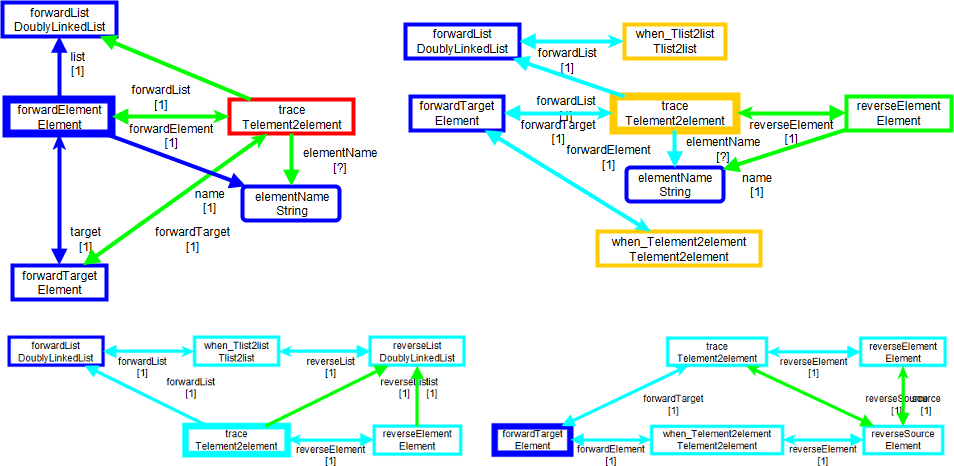
\includegraphics[width=1.0\textwidth]{QVTsMicromappings.png}
	\caption{(Automated) QVTs exposition of element2element with 4 Micromappings.}
	\label{fig:QVTsMicromappings}
\end{figure}

The first micromapping at top left creates the trace object provided the BLUE input pattern can be recognised, but without checking the CYAN dependencies. The speculated trace object is shown in RED to highlight the hazard that all consumers must check the residual CYAN dependencies.

The second micromapping at top right completes the dependency checks and creates the corrolaries.

A corrolary is a GREEN node that can be created without reference to other CYAN nodes once any speculation has been validated. In Fig~\ref{fig:UMLXelement2element}, the GREEN $reverseElement$ is a corrolary of the GREEN $trace$ element. The corresponding $list2list$, not shown, has its $reverseList$ as a corrolary.

In Fig~\ref{fig:QVTselement2element}, four CYAN nodes (and edges) must be satisfied before the GREEN elements are created. Two of the CYAN elements are corrolaries and so it is sufficient to check for successful speculation of the two non-corrolary CYAN external nodes and of the RED internal node. The three orange nodes at the top right of Fig~\ref{fig:QVTsMicromappings} therefore identify the nodes whose speculation must succeed before further execution is permitted.

The third and fourth mappings at the bottom join up the residual references.

In this example we have only trace nodes whose speculation is guaranteed and corrolaries that are guaranteed, allowing the troublesome micromapping step to be statically scheduled. More generally, some awkward predicates may appear at the top right of Fig~\ref{fig:QVTselement2element}. These require a global run-time evaluation; if all predicates are satisfied all related speculations may proceed; if any predicate is not satisfied, no related speculation can be exploited.

The traditional `copy all the nodes' first pass is performed by the first two micromappings. The `copy all the edges' is performed by the last two micromappings. The traditional functionality emerges from the analysis, but without erroneously ignoring predicates that may prohibit execution.   
% that as we shall see can be merged.

\subsection{Heads}\label{Heads}

Each micromapping must be invoked so that all possible matches are considered, so, very naively, the micromapping at the top left of Fig~\ref{fig:QVTsMicromappings} involving four BLUE nodes may require a four dimensional search of the elements of the input model. Consideration of the types of the BLUE nodes allows many candidates to be rejected. Consideration of the navigations allows nearly all candidates to be rejected. For each $Element$ object that is considered as a match for the $forwardElement$ node, we do not need to search for the other objects since they are all resolveable by to-one navigation paths from $forwardElement$. A one-dimensional search of $Element$ types is therefore sufficient to find all matches.

The to-one navigation is so important to efficient scheduling that it is to-one navigation that determines the arrows in QVTs expositions. Transitive analysis of the to-one navigations identifies the minimum number of objects that have to be located to allow all other objects to be identified. These minimum objects are referred to as the heads and are drawn with thick borders in QVTs diagrams. In practice, most micromappings have a single head. Therefore most micromappings can be scheduled in linear time using a one-dimensional loop. The remainder incur often unavoidable non-linear costs.

\subsection{Global scheduling}

We can join the heads, at which micromappings consume objects to the loaders/producers of all these nodes, using a connection to mediate any delays between production and consumption. This results in a graph like Fig~\ref{fig:ExecutionContext} enabling each micromapping to be invoked fairly efficiently for only sensibly typed objects. The ordering of invocations can also be quite sensible. But we can do much better by adding dependency edges from every GREEN element production to every CYAN element consumption. Just one of these is shown in Fig~\ref{fig:ObjectContext}. In practice there are a large number of such edges. Fig~\ref{fig:QVTsPartialDependencies} shows about a third of our simple example. Ellipses show the connections, solid lines show the connection paths to heads, dashed lines those for the further GREEN-CYAN dependencies; orange for node-to-node dependencies, brown for edge-to-edge dependencies.

\begin{figure}[h]
	\centering
	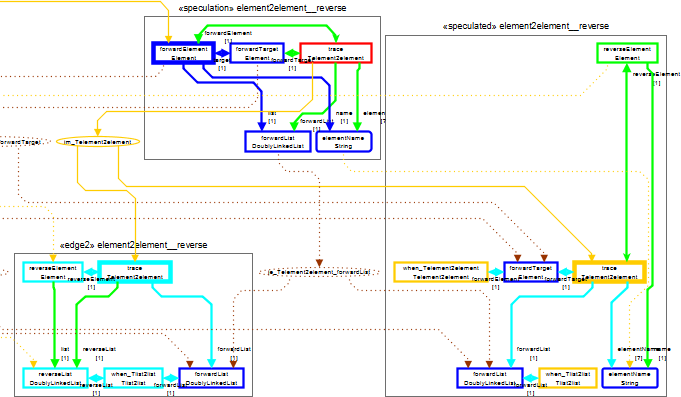
\includegraphics[width=1.0\textwidth]{QVTsFullDependencies.png}
	\caption{(Automated) Partial overall detailed dependencies.}
	\label{fig:QVTsPartialDependencies}
\end{figure}

Once we have extracted the connections and dependencies, we can ignore the internals of each micromapping and use the simpler representation of Fig~\ref{fig:QVTsFullDependencies}. The loader at the top primes two elliptical connections that directly feed four micromapping rectangles which provide outputs for three other micromappings. For these simple single head micromappings the solid lines form a simple call tree with communication buffers. The dashed lines and ellipses identify further communications that do not need to be reified, since production is guaranteed to occur before consumption. Each consuming micromapping can locate the consumed object by navigation from one if its heads. 

\begin{figure}[h]
	\centering
	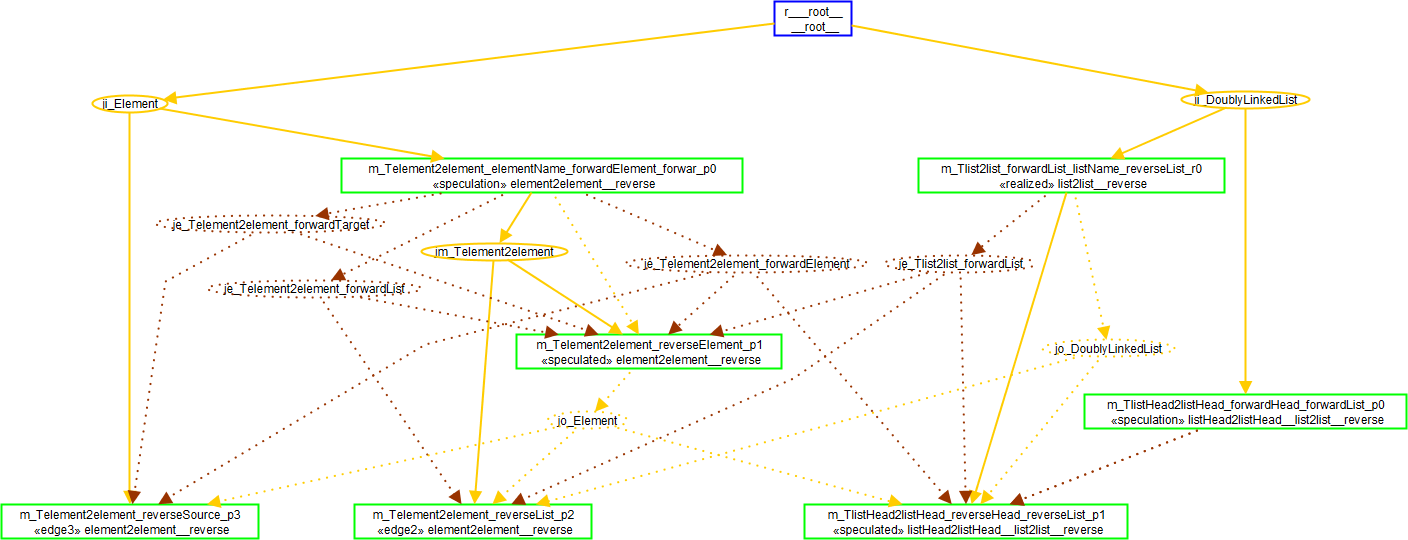
\includegraphics[width=1.0\textwidth]{QVTsDependencies.png}
	\caption{(Automated) Full overall overview dependencies.}
	\label{fig:QVTsFullDependencies}
\end{figure}

So far the micromappings and connections have been very strongly guided by analysis of the transformation and the metamodels. Now we have a potentially NP-complete problem to solve; choose an execution order for the micromappings that minimises run-time overheads; in particular satisfy as many dependencies as possible at compile-time. In practice the graph is mostly acyclic and so there are a small number of relatively similar good solutions and large numbers of bad and truly hideous solutions that can be rejected by heuristics. The current heuristics allocate an integer index to each micromapping in a top down depth first fashion. Within a cycle micromappings have a distinct first and last indexes.

Once each micromapping has an index, or index range, and provided the run-time invokes micromappings in index order, all those dependencies that are inherently satisfied can be pruned. For the running example, all dependencies can be satisfied by the static schedule shown in Fig~\ref{fig:QVTsSchedule}. The indexes are shown at the bottom of each micromapping node.

Optimizations are possible, such as the merge of the micromappings at index 4 and 5. Further optimizations are future work.
% A bottom-up allocation of indexes may enable more micromappings to be merged and so reduce run-time overheads.

\begin{figure}[h]
	\centering
	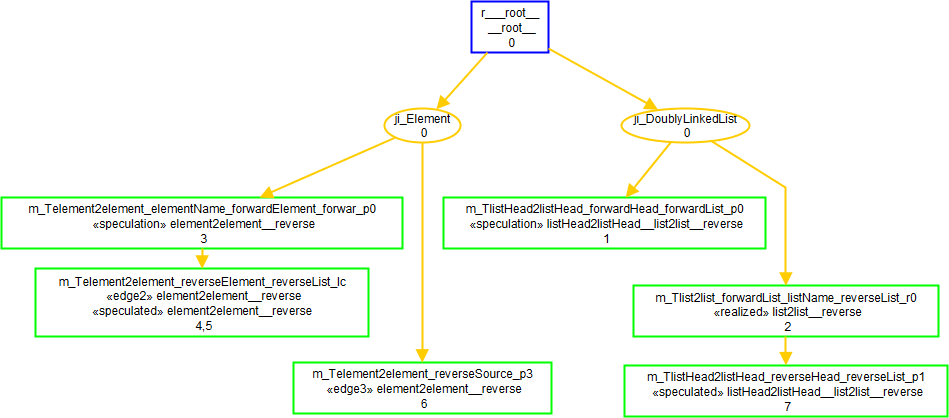
\includegraphics[width=1.0\textwidth]{QVTsSchedule.png}
	\caption{(Automated) Overall schedule.}
	\label{fig:QVTsSchedule}
\end{figure}

\section{Results}\label{Results}

The running example was first presented at the EXE~2016 workshop \cite{Willink-EXE2016}. The performance of Eclipse QVTc and QVTr using interpreted execution and Java code generation was compared with alternative transformation tools. Fig~\ref{fig:DoublyLinkedListReversalPerformance} shows the performance on log-log scales for 100 to 10,000,000 model elements.

\begin{figure}[h]
	\centering
	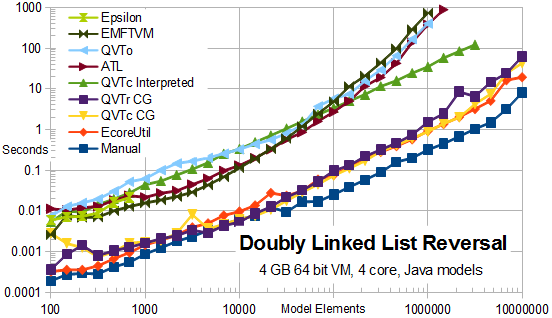
\includegraphics[width=1.0\textwidth]{DoublyLinkedListReversalPerformance.png}
	\caption{Performance of the Doubly Linked List Reversal transformation.}
	\label{fig:DoublyLinkedListReversalPerformance}
\end{figure}

The two fastest results use a fully manually coded and a partially manually coded solution based on the EcoreUtil copier. The results for Eclipse QVTc and QVTr using Java Code Generation are only a little slower.
The corresponding interpreted performance is about 20 times slower. These results scale fairly linear demonstrating that a good declarative schedule was identified.

The curves for ATL, EMTVM and QVTo are similar to QVTc interpreted until a quadratic effect takes over for large models.
Epsilon runs out of stack for comparatively small models.

\section{Related Work}\label{Related Work}

Existing model to model transformation tools such as ATL, Eclipse QVTo, Epsilon and Henshin \cite{Eclipse-Henshin} do very little if any static analysis or optimization. This work on static analysis and optimization of declarative schedules and metamodels using micromappings and connections appears to be almost completely novel. 

In the Triple Graph world, a catalogue of optimizations has been proposed \cite{TGG-Optimization}; domain driven applicability, caching/indexing, static analysis, incremental execution. Many of these come for free in the current work.

The explicit middle model imposed by QVTc traceability reifies a trace object so that to-one navigation paths between source and target can be very cheap and optimized to avoid more expensive paths.
% The use of the 'wrong' domain is not expensive.
The trace object is an inherent cache of related information. Indexing is an OCL-level further work optimization. Local and global analyses for the Micromapping Model of Computation have been described in the preceding sections.

%Incremental execution has not been discussed in this paper. The Connections shown in Fig~\ref{fig:ExecutionContext} are well suited to incremental and concurrent execution.

Although not discussed in this paper, the utility of Connections shown in Fig~\ref{fig:ExecutionContext} for incremental execution is demonstrated by the Eclipse implementation.

Detailed comparison of the approaches is quite hard, since it is very easy to provide a really bad reference implementation against almost any sensible implementation will appear fantastic.

This work diverged from an early Epsilon prototype to exploit the very strong limitations imposed by metamodels and declarative mappings. It therefore uses heuristics to produce a useful schedule relatively quickly, rather than exploring a large number of alternative schedules in an infeasible time \cite{Horacio-planning}.

\section{Status and Further Work}\label{Status}

The approach has evolved from an early Epsilon prototype through rewrites in Java to produce a usable tool. The next rewrite should use QVTr/UMLX as the programming language to further demonstrate their utility and to achieve the benefits of incremental code generation to enhance compilation times.

\paragraph{Acknowledgements}

Many thanks to Adolfo S\'anchez-Barbudo Herrera for helpful comments on a draft, to Horacio Hoyos Rodriguez for the Epsilon prototype and to all Dimitris Kolovos' team for insightful discussions.

\section{Conclusion}\label{Conclusion}

We have introduced the Micromapping Model of Computation involving Micromappings and Connections to provide local and global analyses of a declaration model transformation. 

We have described optimizations that support derivation of an efficient schedule for  QVTc, QVTr and UMLX.

Results of the first optimized code generated implementation show that declarative transformations can approach the performance of manually coded transformations.  
%
% ---- Bibliography ----
%
\begin{thebibliography}{}

\bibitem{TGG-Optimization}
Leblebici, E:, Anjorin, A:, Sch\"urr, A: A Catalogue of Optimization Techniques for Triple Graph Grammars,
In:  Fill,  H.G.,  Karagiannis,  D.,  Reimer,  U.  (eds.)
Modellierung 14. LNI, vol. 225, pp. 225–240. GI (2014)

\bibitem{moc}
Lee, E., Sangiovanni-Vincentelli, A.: Comparing models of computation, Proceedings of the 1996 IEEE/ACM international conference on Computer-aided design

\bibitem{QVT-1.0}
OMG. Meta Object Facility (MOF) 2.0 Query/View/Transformation Specification, Version 1.0.
OMG Document Number: formal/2008-04-03, April 2008.

\bibitem{Horacio-planning}
Rodriguez, H.H:, Kolovos, D: Declarative Model Transformation Execution Planning,
15th International Workshop on OCL and Textual Modeling, Saint-Malo, October 2016

\bibitem{UMLX}
Willink, E: UMLX : A Graphical Transformation Language for MDA
Model Driven Architecture: Foundations and Applications, MDAFA 2003, Twente, June 2003.
\url{http://eclipse.org/gmt/umlx/doc/MDAFA2003-4/MDAFA2003-4.pdf}

\bibitem{Willink-EXE2016}
Willink, E: Local Optimizations in Eclipse QVTc and QVTr using the Micro-Mapping Model of Computation,
2nd International Workshop on Executable Modeling, Exe 2016, Saint-Malo, October 2016.
\url{http://eclipse.org/mmt/qvt/docs/EXE2016/MicroMappings.pdf}

\bibitem{Eclipse-ATL}
Eclipse ATL Project.\\
\url{https://projects.eclipse.org/projects/modeling.mmt.atl}

\bibitem{Eclipse-Henshin}
Eclipse Henshin Project.\\
\url{https://projects.eclipse.org/projects/modeling.emft.henshin}

\bibitem{Eclipse-QVTd}
Eclipse QVT Declarative Project.\\
\url{https://projects.eclipse.org/projects/modeling.mmt.qvtd}

\end{thebibliography}
\end{document}
